\documentclass[11pt, a4paper, dvipdfmx]{jsarticle}
    \usepackage{amsmath}
    \usepackage{amsthm}
    \usepackage[psamsfonts]{amssymb}
    \usepackage{color}
    \usepackage{ascmac}
    \usepackage{amsfonts}
    \usepackage{mathrsfs}
    \usepackage{amssymb}
    \usepackage{graphicx}
    \usepackage{fancybox}
    \usepackage{enumerate}
    \usepackage{verbatim}
    \usepackage{subfigure}
    \usepackage{proof}
    \usepackage{listings}
    \usepackage{otf}
 %
    \theoremstyle{definition}
    %
    %%%%%%%%%%%%%%%%%%%%%%%%%%%%%%%%%%%%%%
    %ここにないパッケージを入れる人は,必ずここに記載すること.
    %
    %%%%%%%%%%%%%%%%%%%%%%%%%%%%%%%%%%%%%%
    %ここからはコード表です.
    %
   \newtheorem{Axiom}{公理}[section]
    \newtheorem{Definition}[Axiom]{定義}
    \newtheorem{Theorem}[Axiom]{定理}
    \newtheorem{Proposition}[Axiom]{命題}
    \newtheorem{Lemma}[Axiom]{補題}
    \newtheorem{Corollary}[Axiom]{系}
    \newtheorem{Example}[Axiom]{例}
    \newtheorem{Claim}[Axiom]{主張}
    \newtheorem{Property}[Axiom]{性質}
    \newtheorem{Attention}[Axiom]{注意}
    \newtheorem{Question}[Axiom]{問}
    \newtheorem{Problem}[Axiom]{問題}
    \newtheorem{Consideration}[Axiom]{考察}
    \newtheorem{Alert}[Axiom]{警告}
    %%%%%%%%%%%%%%%%%%%%%%%%%%%%%%%%%%%%%%
    %
    %定義や定理等に番号をつけたくない場合(例えば定理1.1等)は以下のコードを使ってください.
    %但し,例えば\Axiom*{}としてしまうと番号が付いてしまうので,必ず \begin{Axiom*} \end{Axiom*}の形で使ってください.
    \newtheorem*{Axiom*}{公理}
    \newtheorem*{Definition*}{定義}
    \newtheorem*{Theorem*}{定理}
    \newtheorem*{Proposition*}{命題}
    \newtheorem*{Lemma*}{補題}
    \newtheorem*{Example*}{例}
    \newtheorem*{Corollary*}{系}
    \newtheorem*{Claim*}{主張}
    \newtheorem*{Property*}{性質}
    \newtheorem*{Attention*}{注意}
    \newtheorem*{Question*}{問}
    \newtheorem*{Problem*}{問題}
    \newtheorem*{Consideration*}{考察}
    \newtheorem*{Alert*}{警告}
    \renewcommand{\proofname}{\bfseries Proof}
    
    \newcommand{\A}{\bf 証明}
    \newcommand{\B}{\it Proof}
    
    %
    %%%%%%%%%%%%%%%%%%%%%%%%%%%%%%%%%%%%%%
    %英語で定義や定理を書きたい場合こっちのコードを使うこと.
    \newtheorem{Axiom+}{Axiom}[section]
    \newtheorem{Definition+}[Axiom+]{Definition}
    \newtheorem{Theorem+}[Axiom+]{Theorem}
    \newtheorem{Proposition+}[Axiom+]{Proposition}
    \newtheorem{Lemma+}[Axiom+]{Lemma}
    \newtheorem{Example+}[Axiom+]{Example}
    \newtheorem{Corollary+}[Axiom+]{Corollary}
    \newtheorem{Claim+}[Axiom+]{Claim}
    \newtheorem{Property+}[Axiom+]{Property}
    \newtheorem{Attention+}[Axiom+]{Attention}
    \newtheorem{Question+}[Axiom+]{Question}
    \newtheorem{Problem+}[Axiom+]{Problem}
    \newtheorem{Consideration+}[Axiom+]{Consideration}
    \newtheorem{Alert+}{Alert}
    %\renewcommand{\proofname}{\bfseries 証明}
    %
    %
    %%%%%%%%%%%%%%%%%%%%%%%%%%%%%%%%%%%%%%
    %数
    \newcommand{\N}{\mathbb{N}}
\newcommand{\Z}{\mathbb{Z}}
\newcommand{\R}{\mathbb{R}}
\newcommand{\C}{\mathbb{C}}
\newcommand{\W}{{\cal W}}
\newcommand{\cS}{{\cal S}}
\newcommand{\Wpm}{W^{\pm}}
\newcommand{\Wp}{W^{+}}
\newcommand{\Wm}{W^{-}}
\newcommand{\p}{\partial}
\newcommand{\Dx}{D_{x}}
\newcommand{\Dxi}{D_{\xi}}
\newcommand{\lan}{\langle}
\newcommand{\ran}{\rangle}
\newcommand{\pal}{\parallel}
\newcommand{\dip}{\displaystyle }
\newcommand{\e}{\varepsilon}
\newcommand{\dl}{\delta}
\newcommand{\pphi}{\varphi}
\newcommand{\ti}{\tilde}
    \title{単調劣モジュラ関数最大化問題と貪欲法}
    \author{数理科学科 2回生 小泉 孝弥}
    \date{}
\begin{document}
\maketitle
%ソースコードの設定
\lstset{
  basicstyle={\ttfamily},
  identifierstyle={\small},
  commentstyle={\smallitshape},
  keywordstyle={\small\bfseries},
  ndkeywordstyle={\small},
  stringstyle={\small\ttfamily},
  frame={tb},
  breaklines=true,
  columns=[l]{fullflexible},
  numbers=left,
  xrightmargin=0zw,
  xleftmargin=3zw,
  numberstyle={\scriptsize},
  stepnumber=1,
  numbersep=1zw,
  lineskip=-0.5ex
}
\section{初めに}
みなさんは「最適化問題 (Optimization Problem)」という言葉を聞いたことはないだろうか? 
例えば, ナップザック問題(Knapsack Problem), 巡回セールスマン問題(Traveling Salesman Problem) それに加えて
最近話題の機械学習(Machine Learning)も広い意味では最適化問題である. 今回の方程では「劣モジュラ性」という
性質を持った関数の最適化問題を考えて行くことにする. この方程で仮定する知識は1回生レベルの「集合と写像」に関する知識である.\\ \indent
 また, この方程では特に断りのない限り$V$を有限集合とし, 以下の定理は証明をせず用いる.
 \begin{Theorem+}
    $V$, $W$$\subset\R$を有限集合とし, $f$を$V$から$W$への写像とする. この時$f$には最大値が存在する.
 \end{Theorem+}
 \begin{Definition+}(argmax)\\
     $V$, $W$$\subset\R$を集合とし, $f$を$V$から$W$への写像とする. この時の写像$f$の最大値を$\alpha$とする. この時
     最大点集合$\mathop{\rm arg~max}\limits f$を以下のように定義する. 
     \begin{align*}
        \mathop{\rm arg~max}\limits f = \{x\in V~|~ f(x) = \alpha\}
     \end{align*}
    \end{Definition+}
    また任意の有限集合$S$に対して$|S|$で集合$S$の要素数を表す.    
\section{劣モジュラ関数}
まず劣モジュラ関数を定義して行く.
\begin{Definition+}(集合関数)\\
   $f$をVの冪集合$2^{V} = \{S~|~S\subset V\}$から$\R$への写像とする. この時$f$を集合関数と呼ぶ.
\end{Definition+}
\begin{Definition+}(離散微分)\\
    $f$を集合関数とする. $S$を$V$の部分集合とし$e$を$V$の元とする. この時$f$の$S$での
    離散微分(Discreate derivative)を
    \begin{align*}
        \Delta_{f}(e | S) := f(S\cup\{e\}) - f(S)
    \end{align*}
    と定義する.
\end{Definition+}
\begin{Definition+}(劣モジュラ関数)\\
    $f$を集合関数とする. $f$が劣モジュラ関数(Submodular function)であるとは
    \begin{align*}
        \forall A, B\subset V, \forall e\in V, ~(A\subset B かつe\in V - B)\Longrightarrow \Delta_{f}(e | A)\geq\Delta_{f}(e | B)
    \end{align*}
    を満たすことをいう.
\end{Definition+}
\begin{Theorem+}$f$を集合関数とする. この時
    \begin{enumerate}
        \item $f$は劣モジュラ関数である.
        \item $\forall A, B\subset V, f(A\cap B) + f(A\cup B)\leq f(A) + f(B)$ 
    \end{enumerate}
    は同値である.
    \begin{proof}
        1.$\implies$2.) 任意に$A, B\subset V$をとる. $A - B = \phi$の時, すなわち
        $A\subset B$の時は$A\cap B = A$, $A\cup B = B$より成立する. そこで, $A - B\neq\phi$の時を考える.
        $| A - B| = m$とし$A - B = \{i_{1}, i_{2}, \cdots, i_{m}\}$とする. $A_{0} = A\cap B$, $B_{0} = B$として
        $A_{k}, B_{k} (k\in\{1, 2, \cdots, m\})$を以下のように定義する.
        \begin{align*}
            A_{1} = A_{0}\cup\{i_{1}\}, ~~~~~ A_{2} = A_{0}\cup\{i_{1}, i_{2}\}, \cdots, ~~~~~ A_{m} = A_{0}\cup\{i_{1}, i_{2}, \cdots, i_{m}\}\\
            B_{1} = B_{0}\cup\{i_{1}\}, ~~~~~ B_{2} = B_{0}\cup\{i_{1}, i_{2}\}, \cdots, ~~~~~ B_{m} = B_{0}\cup\{i_{1}, i_{2}, \cdots, i_{m}\}
        \end{align*}
        この時$A_{m} = A$, $B_{m} = A\cup B$である. また各$k\in\{1, 2, \cdots, m\}$に対して
        \begin{align*}
             A_{k - 1}\subset B_{k-1}かつA_{k} = A_{k-1}\cup\{i_{k}\}かつB_{k} = B_{k-1}\cup\{i_{k}\}
        \end{align*}
        が成立するので1.より
        \begin{align*}
            \forall k\in\{1, 2, \cdots, m\}, f(A_{k}) - f(A_{k - 1})\geq f(B_{k}) - f(B_{k-1})
        \end{align*}
        が成立する. $k$についてこの不等式の両辺の和をとると, 
        \begin{align*}
            \sum_{k =1}^{m}\left(f(A_{k}) - f(A_{k - 1})\right)\geq\sum_{k =1}^{m}\left(f(B_{k}) - f(B_{k - 1})\right)
        \end{align*}
        両辺を計算すると
        \begin{align*}
            f(A_{m}) - f(A_{0})\geq f(B_{m}) - f(B_{0})
        \end{align*}
        となる. $A, B$は任意なので$A_{m} = A$, $B_{m} = A\cup B$, $B_{0} = B$より
        \begin{align*}
            \forall A, B\subset V, f(A\cap B) + f(A\cup B)\leq f(A) + f(B)
        \end{align*}
        が成立する.\\

        2.$\implies$1.) 任意に$A, B\subset V$と$i\in V - B$を$A\subset B$となるようにとる. $A^{'} = A\cup \{i\}, B^{'} = B$とすると2.より
        \begin{align*}
            f(A^{'}) + f(B^{'})\geq f(A^{'}\cup B^{'}) + f(A^{'}\cap B^{'})
        \end{align*}
        が成立する. ここで$A^{'}\cup B^{'} = B\cup\{i\}$, $A^{'}\cap B^{'} = A$であることから
        \begin{align*}
            f(A^{'}) + f(B^{'})\geq f(B\cup\{i\}) + f(A)
        \end{align*}
        $A^{'}, B^{'}$の定義より
        \begin{align*}
            f(A\cup \{i\}) + f(B)\geq f(B\cup\{i\}) + f(A)
        \end{align*}
        式を整理すると
        \begin{align*}
            f(A\cup \{i\}) - f(A)\geq f(B\cup\{i\}) + f(B)
        \end{align*}
        したがって, $A, B\subset V$と$i\in V - B$は任意だったので,
        \begin{align*}
            \forall A, B\subset V, \forall e\in V,A\subset B かつe\in V - B\Longrightarrow \Delta_{f}(e | A)\geq\Delta_{f}(e | B)
        \end{align*}
        したがって, $f$は劣モジュラ関数である.
    \end{proof}
\end{Theorem+}
\begin{Definition+}(単調)\\
    $f$を集合関数とする. $f$が単調(Monotone)であるとは
    \begin{align*}
        \forall S, T\subset V, S\subset T\Longrightarrow f(S)\leq f(T)
    \end{align*}
    を満たすことを言う.
\end{Definition+}
\begin{Theorem+}
    $f$を集合関数とする.このとき
    \begin{enumerate}
        \item $f$が単調である.
        \item $\forall S\subset V, \forall e\in V, \Delta_{f}(e | S)\geq 0$
    \end{enumerate}
    は同値である.
    \begin{proof}
        証明は読者への演習問題とする.
    \end{proof}
\end{Theorem+}
\begin{Theorem+}
    $f_{1}, f_{2}, f$を劣モジュラ関数 . $\alpha$を正の実数とする. この時
    \begin{enumerate}
        \item $f_{1} + f_{2} $ は劣モジュラ関数.
        \item $\alpha f$は劣モジュラ関数.
    \end{enumerate}
    が成立する.
    \begin{proof}
        任意に$V$の部分集合$A$, $B$と$V$の元$e$をとる. $A\subset B$, $e\in V - B$と仮定する.\\
        1. $f_{1}$, $f_{2}$は劣モジュラ関数 だから
        \begin{align*}
            \Delta_{f_{1}}(e|A)\geq \Delta_{f_{1}}(e|B)
        \end{align*}
        \begin{align*}
            \Delta_{f_{2}}(e|A)\geq \Delta_{f_{2}}(e|B)
        \end{align*}
        が成立する. 両辺を足すと
        \begin{align*}
            \Delta_{f_{1}}(e|A) + \Delta_{f_{2}}(e|A)\geq \Delta_{f_{1}}(e|B) + \Delta_{f_{2}}(e|B)
        \end{align*}
        したがって
        \begin{align*}
            \Delta_{f_{1} + f_{2}}(e|A)\geq \Delta_{f_{1} + f_{2}}(e|B)
        \end{align*}
        したがって, $f_{1} + f_{2}$は劣モジュラ関数である.\\
        2. $\alpha > 0$を任意にとる. $f$は劣モジュラ関数であるので
        \begin{align*}
            \Delta_{f}(e|A)\geq \Delta_{f}(e|B)
        \end{align*}
        両辺を$\alpha > 0$倍すると
        \begin{align*}
            \alpha\Delta_{f}(e|A)\geq \alpha\Delta_{f}(e|B)
        \end{align*}
        したがって
        \begin{align*}
            \Delta_{\alpha f}(e|A)\geq \Delta_{\alpha f}(e|B)
        \end{align*}
        したがって$\alpha f$ は劣モジュラ関数である.
     \end{proof}
\end{Theorem+}
\begin{Definition+}(単調劣モジュラ関数)\\
    集合関数$f$が劣モジュラかつ単調であるとき$f$を単調劣モジュラ関数(Monotone Submodular function)と言う.
\end{Definition+}
\section{単調劣モジュラ関数最大化問題と貪欲法}
この節では$f$を非負の単調劣モジュラ関数とする.
\subsection{単調劣モジュラ関数最大化問題}
 前節では劣モジュラ関数の定義および様々な性質を述べてきた. この節での目的は単調劣モジュラ関数を
 ある条件のもと最大化\footnote{ここでの最大化とは出来るだけ関数の最大値に近づくような手法のことであり, 実際に関数の最大値が出る保証はない.}する$V$の部分集合
 $S$を見つけるアルゴリズムを与えることである.
 そして, この節では特に集合
 \begin{align*}
    \{ f(S)~|~S\subset V\text{ and }|S| \leq k\}
 \end{align*} 
 が最大値をとるときの$V$の部分集合$S$を見つけることが目標である(そのような$S$を最適解と呼ぶ). また$k$は$0<k\leq |V|$を満たす定数である. 
 この問題をこの方程では単調劣モジュラ関数最大化問題(Submodular function maximization problem)と呼ぶことにする. 

 \subsection{近似アルゴリズム}
単調劣モジュラ関数最大化問題を解決するための手法について述べる. 
まず, 最初に全探索アルゴリズムを考える. これは「制約下でのあらゆる可能性を全て探索する\footnote{実装はbit全探索というものをよく用いる}」アルゴリズムである. 
このアルゴリズムであれば確実に解が出せるので単調劣モジュラ関数最大化問題を解決することができる. 
しかしながら, このアルゴリズムでは$V$の部分集合全てを調べる必要があるため$2^{|V|}$回の計算を行う必要がある.(簡単のため$k = |V|$とした.)
$y = 2^x$という関数は以下のグラフ1を見れば分かる通り$x$がある程度大きくなると$y$は非常な大きな値となる. 
これではいくらコンピュータを用いたとしても解くのは不可能である. そこで単調劣モジュラ関数最大化問題の真の解を求めることを諦め,
近似解を求めるために「近似アルゴリズム」というものを利用する. 
\begin{Theorem+}
    単調劣モジュラ関数最大化問題には最適解が存在する.
\begin{proof}
    ${\bf Theorem 1.1.}$より言える.
\end{proof}
これ以降単調劣モジュラ関数最大化問題の最適解を$S_{OPT}$と表記する.
\end{Theorem+}
\begin{Definition+}(近似アルゴリズム)\\
    以下の2つのことを満たすアルゴリズム$\mathcal{A}$を近似アルゴリズムと呼ぶ.
    \begin{enumerate}
        \item $\mathcal{A}$によって近似解が多項式時間\footnote{この方程では多項式時間アルゴリズムの明確な定義はしない. 簡単に説明するならある程度実用的な速さで問題の解が求まるアルゴリズムと思ってもらえれば良い. }で得られる.
        \item $S_{OPT}$と$\mathcal{A}$によって得られる近似解$S_{\mathcal{A}}$の$f$の値の比が一定値より高くなることが理論的に保証される.
    \end{enumerate}
\end{Definition+}
\begin{Theorem+}
    近似アルゴリズム$\mathcal{A}$によって得られる近似解$S_{\mathcal{A}}$とする. この時
    \begin{align*}
        f(S_{\mathcal{A}})\leq f(S_{OPT})
    \end{align*}
    が成立する.
    \begin{proof}
        最大値の定義より言える.
    \end{proof}
\end{Theorem+}
近似アルゴリズムが与えられた時, そのアルゴリズムが良い近似アルゴリズかどうか判定するのには色々な
ものがある. その一つに近似アルゴリズムが最適解にどれだけ近い値を出せているのかというものが考えられる. そこで近似率というものを定義する.
\begin{Definition+}(近似率)\\
    $ 0< \alpha \leq 1$と定数とし, 近似アルゴリズム$\mathcal{A}$によって得られる近似解$S_{\mathcal{A}}$とする. 
    \begin{align*}
        f(S_{\mathcal{A}})\leq \alpha(S_{OPT})
    \end{align*}
    が成立する最大の$\alpha$を$\mathcal{A}$の近似率と呼ぶ.
\end{Definition+}
\begin{figure}[h]
    \centering
    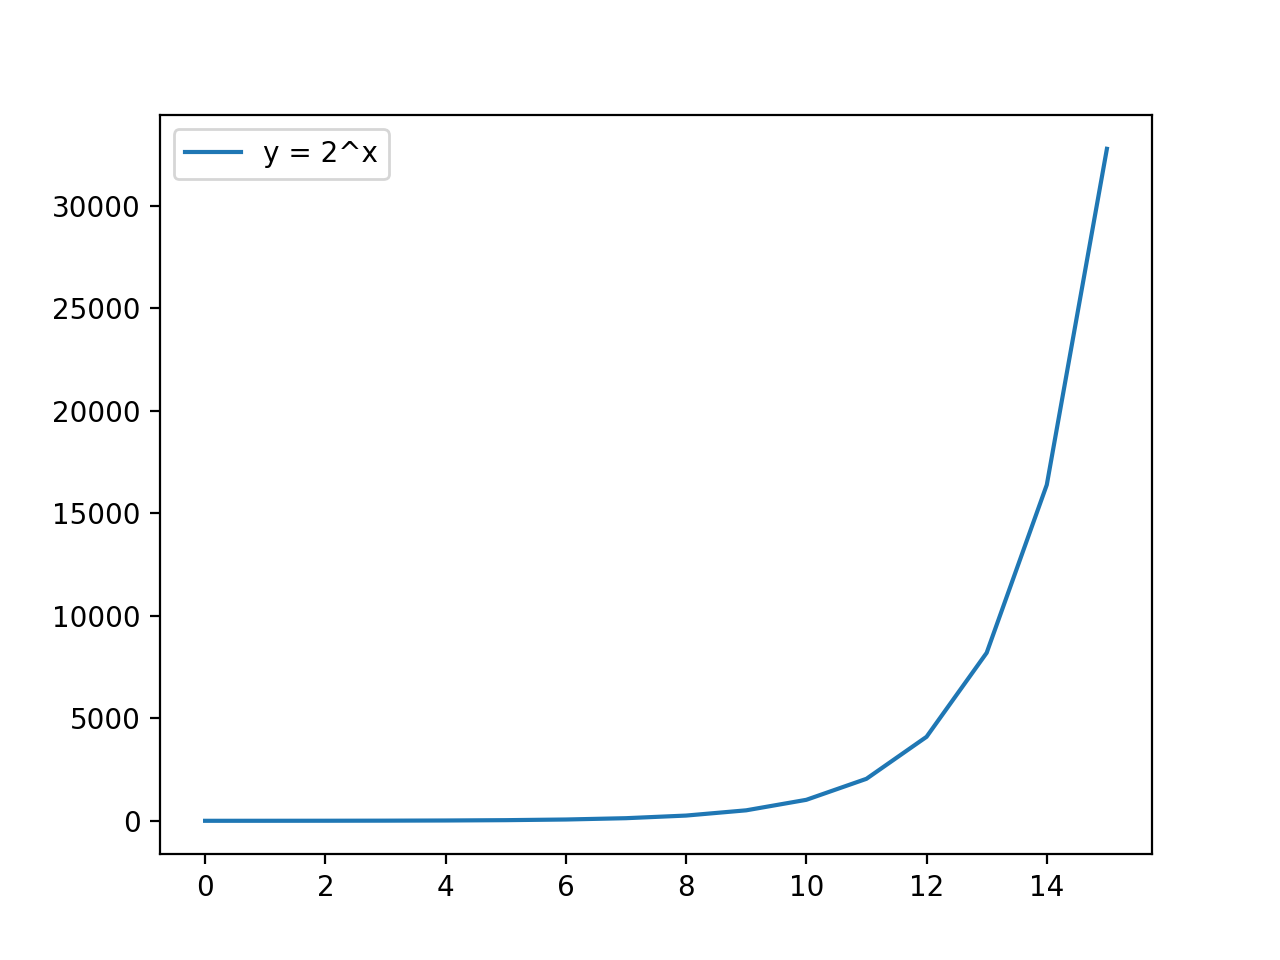
\includegraphics[width = 100mm]{Graph1_houtei.png}
    \caption{グラフ1}
\end{figure}
\subsection{貪欲法}
 今回は単調劣モジュラ関数最大化問題を解くための近似アルゴリズムとして貪欲法(Greedy algorithm)というアルゴリズムを利用する. 貪欲法とは
「その場における最適な解を選択する」というアルゴリズムである. 今回の問題においては
\begin{align*}
    S_{i} = S_{i - 1}\cup\mathop{\rm arg~max}\limits_{e\in V}\Delta_{f}(e~|~S_{i - 1})\hspace{15pt}(S_{0} = \phi)
\end{align*}
を満たす$V$の部分集合列$S_{1}$, $S_{2}$, $\cdots$, $S_{k}(0<k\leq |V|)$を決定することに他ならない. ただし, $\mathop{\rm arg~max}\limits_{e\in V}\Delta_{f}(e~|~S_{i - 1})$の元が2つ以上の場合はどれか一つを選ぶものとする. 
また、このアルゴリズムは多項式時間アルゴリズムである. (本方程では多項式時間アルゴリズムの明確な定義はしていないためこの主張は証明をせず認めることにする.) 
\begin{Proposition+}
$S_{1}$, $S_{2}$$\cdots$, $S_{k}$を貪欲法によって選ばれた$V$の部分集合列とする. この時
    \begin{align*}
        f(S_{1})\leq f(S_{2})\leq \cdots \leq f(S_{k})
    \end{align*}
    が成立する.
    \begin{proof}
        $S_{1}\subset S_{2}\subset \cdots S_{k}$ と$f$の単調性より言える.
    \end{proof}
\end{Proposition+}

\subsection{貪欲法の近似率}
いよいよ本方程の主定理である貪欲法の近似定理\footnote{この名前は著者が勝手につけたものである.}についてのべて行く.
\begin{Lemma+}
    $f$を劣モジュラ関数とする. この時
    \begin{align*}
        \forall S, T\subset V,~ S\subset T\implies f(S) - f(T)\leq \sum_{e\in T - S}\Delta_{f}(e|S)
    \end{align*}
    が成立する.
\end{Lemma+}
\begin{Lemma+}
    $S_{1}$, $S_{2}$$\cdots$, $S_{k}$を貪欲法によって選ばれた$V$の部分集合列とする. この時任意の$l\in\{0, 1, 2, \cdots, k - 1\}$
    に対して 
    \begin{eqnarray*}
          f(S_{l + 1}) -f(S_{l})&\geq& \frac{1}{|S_{OPT} - S_{l}|}(f(S_{OPT}) - f(S_{l})) \\
                                                               &\geq& \frac{1}{k}(f(S_{OPT}) - f(S_{l}))
    \end{eqnarray*}
    が成立する.
\end{Lemma+}
この二つの補題の証明については参考文献の[1]番や[2]番を見て欲しい.
\begin{Lemma+}
    \begin{align*}
        \forall x\in\R, ~1 - x\leq e^{-x}
    \end{align*}
    が成立する.
\end{Lemma+}
%主定理
\begin{Theorem+}(貪欲法の近似定理, Nemhauser)\\
    $S_{1}$, $S_{2}$$\cdots$, $S_{k}$を貪欲法によって選ばれた$V$の部分集合列とする. この時
    \begin{align*}
        \forall l\in\{1, 2, \cdots, k\}, ~f(S_{l}) \geq\left (1 - e^{-\frac{l}{k}}\right)f(S_{OPT})
    \end{align*}
    が成立する. 
    \begin{proof}
         $l\in\{0, 1, 2, \cdots, k - 1\}$を任意にとり, 各$i\in\{0, 1, 2, \cdots, k - 1\}$に対して$\delta_{i} = f(S_{OPT}) - f(S_{i})$ とする. すると
         ${\bf Lemma 3.7.}$より
        \begin{align*}
            \delta_{l+1}\leq\left(1 - \frac{1}{k}\right)\delta_{l}
        \end{align*}
        である. この不等式と$f$の非負性より$\delta_{0} = f(S_{OPT}) - f(\phi)\leq f(S_{OPT})$であることと, ${\bf Lemma 3.8.}$を用いれば
        \begin{align*}
            \delta_{l}\leq \left(1 - \frac{1}{k}\right)^{l}\delta_{0}\leq e^{-\frac{l}{k}}f(S_{OPT})
        \end{align*}
        が従う. $\delta_{l}$の定義より
        \begin{align*}
            f(S_{l}) \geq\left (1 - e^{-\frac{l}{k}}\right)f(S_{OPT})
        \end{align*}
        が成立する.
    \end{proof}
\end{Theorem+}
この定理より貪欲法が近似アルゴリズムであることと, 貪欲法の近似率が $1 - \frac{1}{e} \approx 0.62$ということがわかる.
\section{応用例}
ここでは単調劣モジュラ関数の応用例について紹介をする. 詳細については参考文献を見て欲しい.
\begin{itemize}
    \item 口コミ効果最大化
    \item 文章要約問題
    \item センサー配置問題
    \item 施設の配置問題
    \item 機械学習
\end{itemize}
このように単調劣モジュラ関数には様々な応用がある. 今回紹介した「(個数制約下での)単調劣モジュラ関数最大化問題」の他にも,
ナップザック制約下での単調劣モジュラ関数最大化問題, マトロイド制約下での単調劣モジュラ関数最大化問題などがある. また単調劣モジュラ関数最小化問題
というものもある. 興味のある読者は調べてみると面白いかもしれない.
\section{終わりに}
今回の方程では私が学びたい分野である数理情報学の入門として「単調劣モジュラ関数最大化問題」を2018年度の題材とさせていただいた. 
書き終わってみれば「多項式時間アルゴリズム」などの計算機科学への知識が足りず厳密な議論ができなかったことや応用例の詳細について書けなかったのが
心残りである. 今回は初めてセミナーなしで数学書を読んだので, 改めてセミナーの重要性を感じることができた. 最後にここまで僕のセミナー
に付き合ってくれた全ての先輩や同期に感謝を申し上げるとともに, 2018年度の方程を完了とする.






\begin{thebibliography}{10}
    \bibitem{キー1} 劣モジュラ最適化と機械学習・河原 吉伸,  永野 清仁・2015
    \bibitem{キー2} https://las.inf.ethz.ch/files/krause12survey.pdf・Andreas Krause, Daniel Golovin
    \bibitem{キー3} https://www.openu.ac.il/personal\verb|_|sites/moran-feldman/publications/Handbook2018.pdf・Niv Buchbinder, Moran Feldman
    \bibitem{キー4} https://repository.upenn.edu/cgi/viewcontent.cgi?article=2034\verb|&|context=cis\verb|_|reports・Jennifer Gillenwater
    \bibitem{キー5} http://imi.kyushu-u.ac.jp/~kamiyama/opt2012\verb|_|ppt/nagano.pdf・永野 清仁・2012
    \bibitem{キー6} https://www.youtube.com/watch?v=Z7eMzSHGGAE\verb|&|t=24s・アルゴリズムが世界を変える 3.0
  \end{thebibliography}
\end{document}
